\documentclass[11pt]{article}

\usepackage{bmpsize}
\usepackage[pdftex]{graphicx}
\usepackage{amsmath}
\usepackage{amssymb}
\usepackage{amsthm}
\usepackage{fancyhdr}
\usepackage[margin=2.5cm]{geometry}
\newcommand{\Ohm}{\Omega}
\newcommand{\inv}{^{-1}}
\renewcommand{\part}[1] {\vspace{.10in} {\bf (#1)}}


\pagestyle{fancyplain}


\begin{document}
\title{Interferometry Lab}
\author{David Galbraith}
\maketitle
%COMMENT: In Latex, using the maketitle function will perform all the formatting
%you had set up in the code below in a standard fashion

\normalsize
\begin{abstract} 
In this lab, we did stuff. Hooray! %TODO figure out stuff
\end{abstract}
%COMMENT: It is customary to use the abstract environment for the
%abstract, and to not include a pagebreak after the abstract prior to
%the introduction in a scientific paper


\lhead{\fancyplain{}{\textbf{Lab 2}}}      % Note the different brackets!
\rhead{\fancyplain{}{David Galbraith}}
\medskip                        % Skip a "medium" amount of space
                                % (latex determines medium is)
                                % Also try: \bigskip, \littleskip

\thispagestyle{plain}

\section{Introduction}
%COMMENT: Sections and subsections have their own format that will make
%the divisions in what you wrote more clear, and will number themselves,
%allowing you to focus more on content rather than order


\section{Experiments, Observations, Analysis and Interpretation} 

\subsection{Calculating When Objects of Interest are Overhead}
The first thing we had to do in order to observe the celestial bodies was to figure out when they would be visible. Given the right ascensions and declinations of the various objects, we used rotation matrices to calculate altitude and azimuth for various local sidereal times in Berkeley. When the calculated altitudes are positive, the object is visible, disregarding the view-blocking tendencies of the Berkeley hills and surrounding buildings. To calculate the altitude and azimuth given right ascension and declination, you use the formulas $A = \tan\inv{\sin{h}/(\cos{h}\sin{\phi_o} - \tan{\delta}\cos{\phi_o})}$ and $a = \sin\inv{\sin{\phi_o}\sin{\delta} + \cos{\phi_o}\cos{\delta}\cos{h}}$ where $A$ is the azimuth, $h$ is the hour angle, $\phi_o$ is the latitude of the observer, $\delta$ is the declination, and $a$ is the altitude. These equations are derived from the equation 
$\begin{bmatrix}
\sin{\phi_o} & 0 & -\cos{\phi_o} \\
0 & 1 & 0 \\
\cos{\phi_o} & 0 & \sin{\phi_o}
\end{bmatrix}
\begin{bmatrix}
\cos{\delta}\cos{h} \\
\cos{\delta}\sin{h}
\sin{\delta}
\end{bmatrix}
=
\begin{bmatrix} 
\cos{a}\cos{A} \\
\cos{a}\sin{A} \\
\sin{a}
\end{bmatrix}$

which is where the rotation matrices come in. The code used to calculate the altitudes and azimuths apppears in rotation.py; the resulting LSTs of visibility appear in Table \ref{lsts}. These methods don't work on the sun and the moon because they are too close to the earth to have static right ascension and declination. Luckily, one can determine when they are visible by looking outside.

\begin{figure}
\centering
\begin{tabular}{c|c}
Celestial Object & LST interval of visibility (radians) \\
W3 & [0, 2$\pi$] \\
Crab nebula & [5.85, 3.35] \\
Orion & [6.25, 2.97] \\
3C274 & [1.41, 4.89] \\
M17 & [3.46, 6.15] \\
W43 & [3.63, 6.21] \\
W49 & [3.31, .42] \\
W51 & [3.30, .56] \\
3C405 & [3.6, .574] \\
3C461 & [0, 2$\pi$]
\end{tabular}
\caption{When the objects are visible in LST radians. \label{lsts}}
\end{figure}

\subsection{The Sun}
Then, we looked at the sun. First we looked at it for an hour to make sure our scripting was functional, and then we looked at it for an entire day. The hour-long measurements appear in Figure \ref{hoursun} and the day measurements appear in Figure \ref{daysun}.

\begin{figure}
\centering
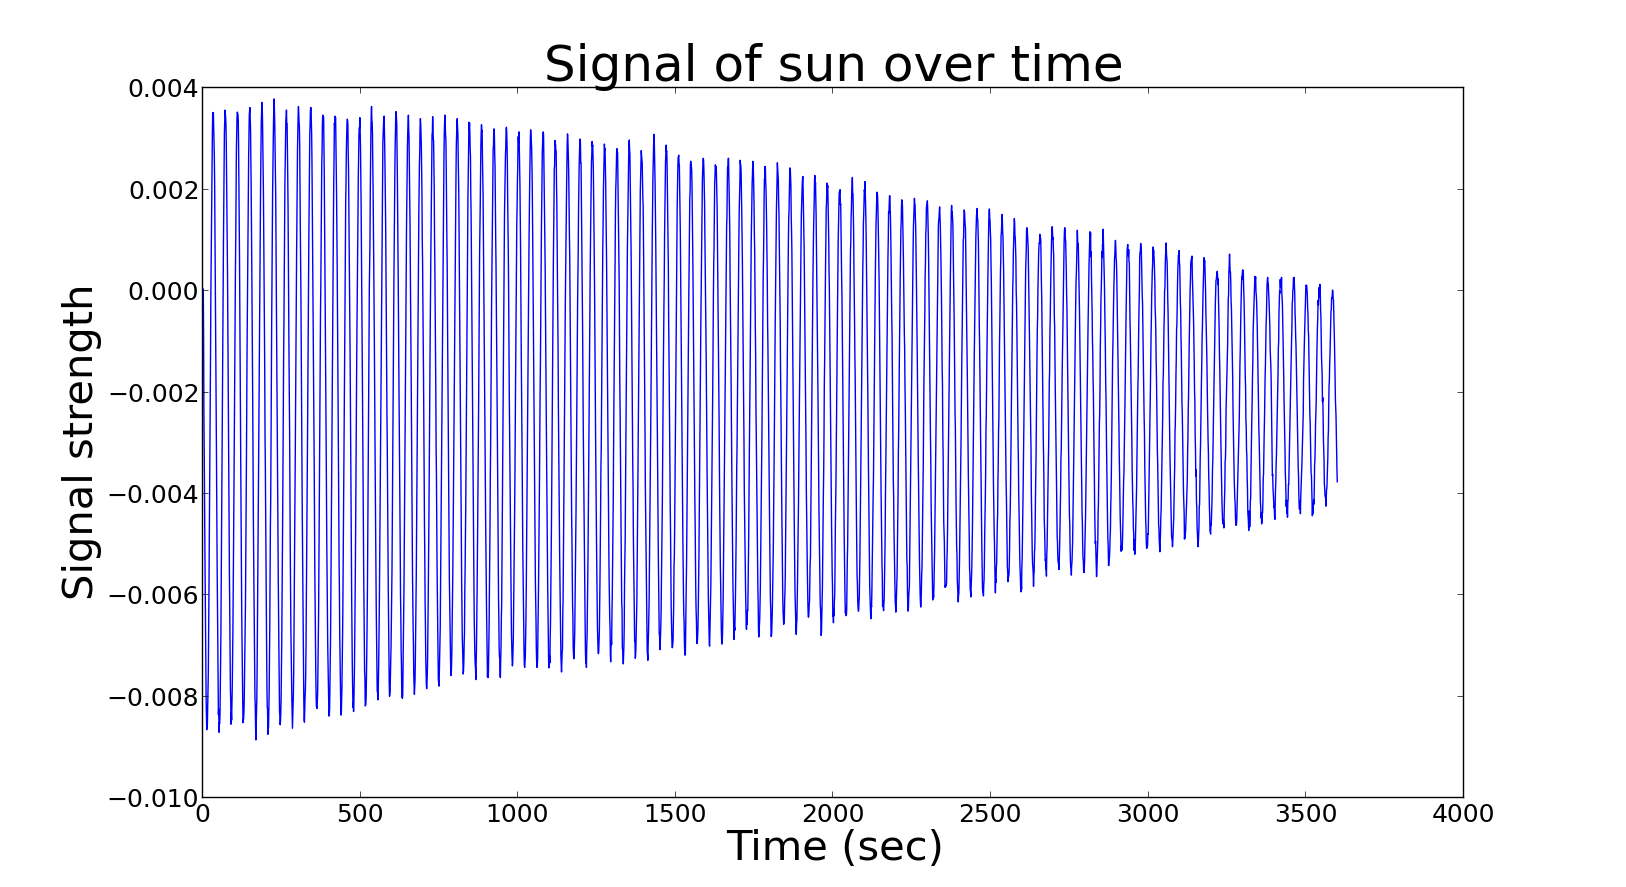
\includegraphics[scale=0.35]{garphs/sunhourvolt}
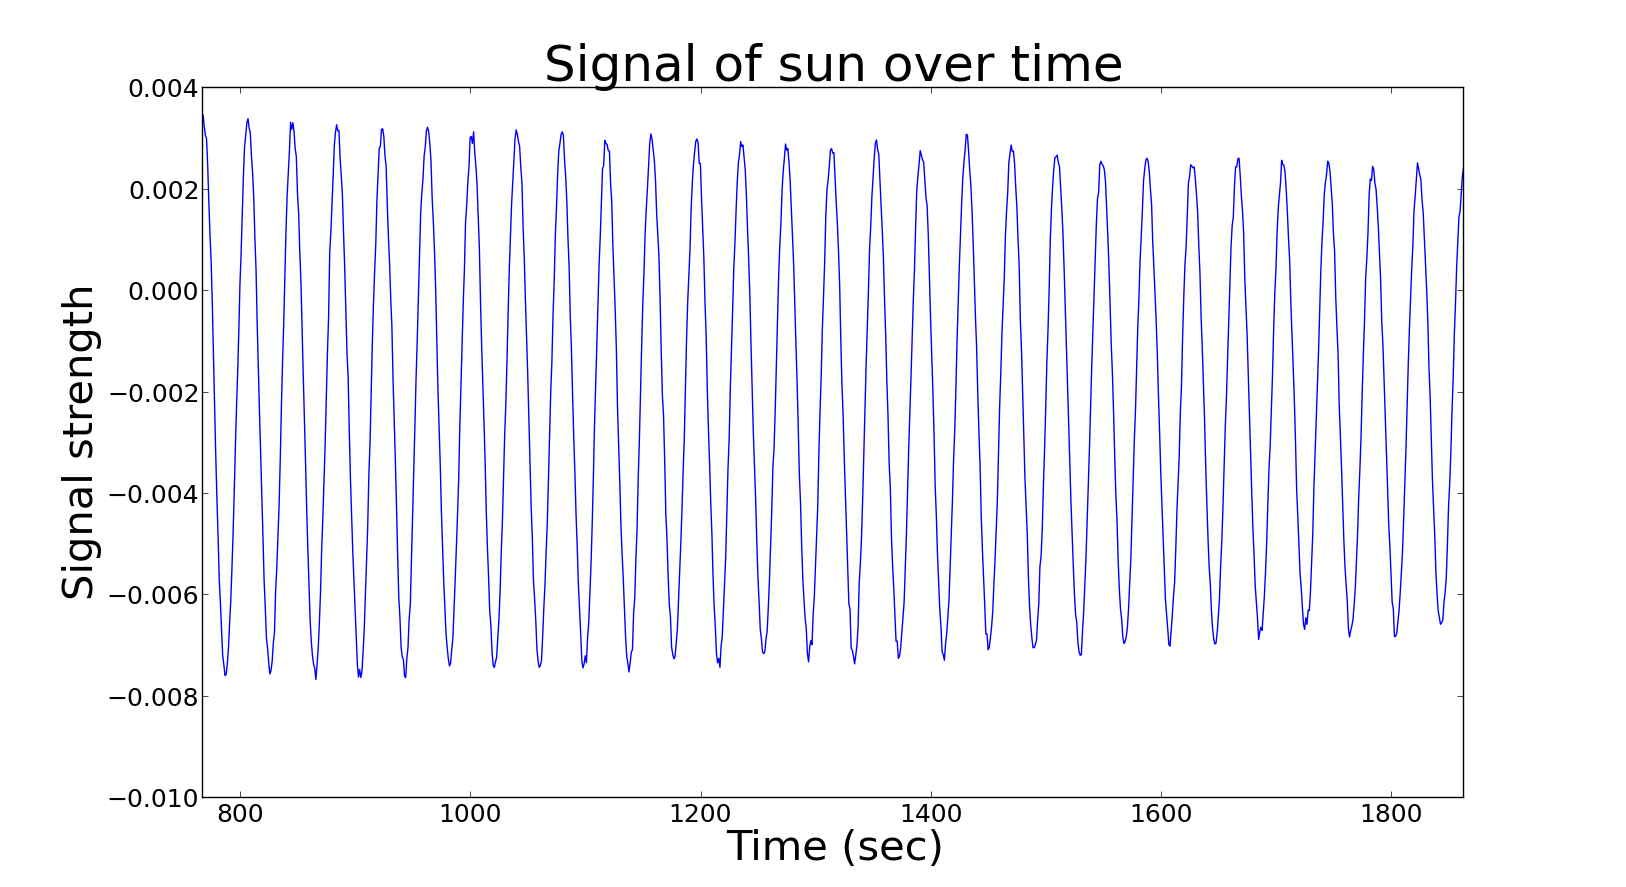
\includegraphics[scale=0.35]{garphs/sunhourzoom}
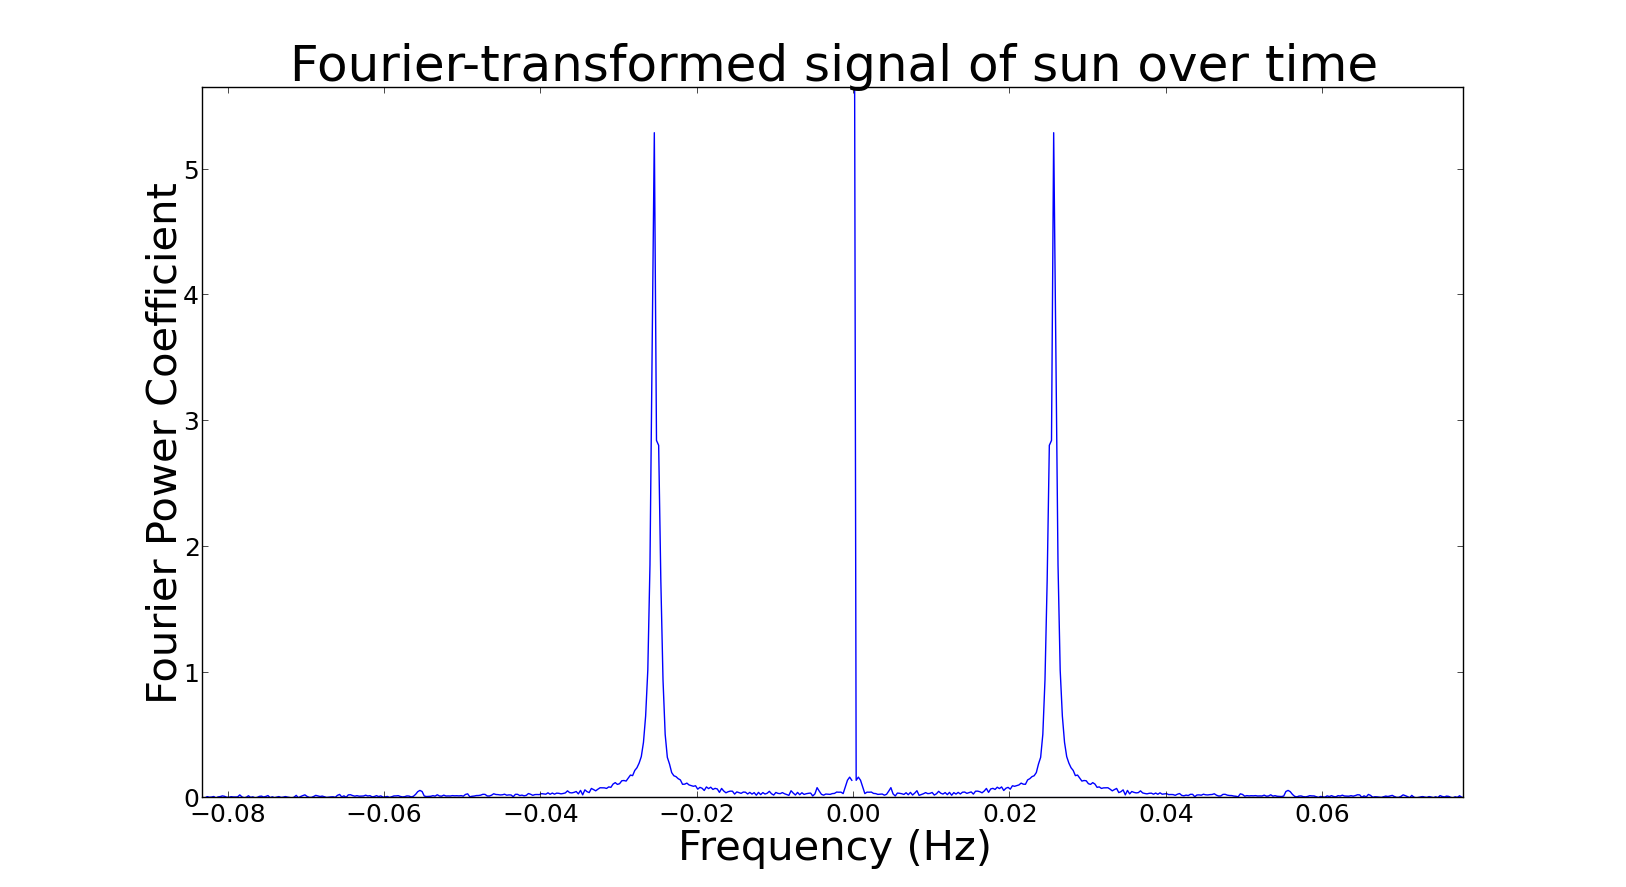
\includegraphics[scale=0.35]{garphs/sunhourfourier}
\caption{The top graph shows the signals we measured from the sun over an hour. The middle shows a zoomed-in version of this data. The bottom shows the Fourier transform of the top. \label{hoursun}}
\end{figure}

\begin{figure}
\centering
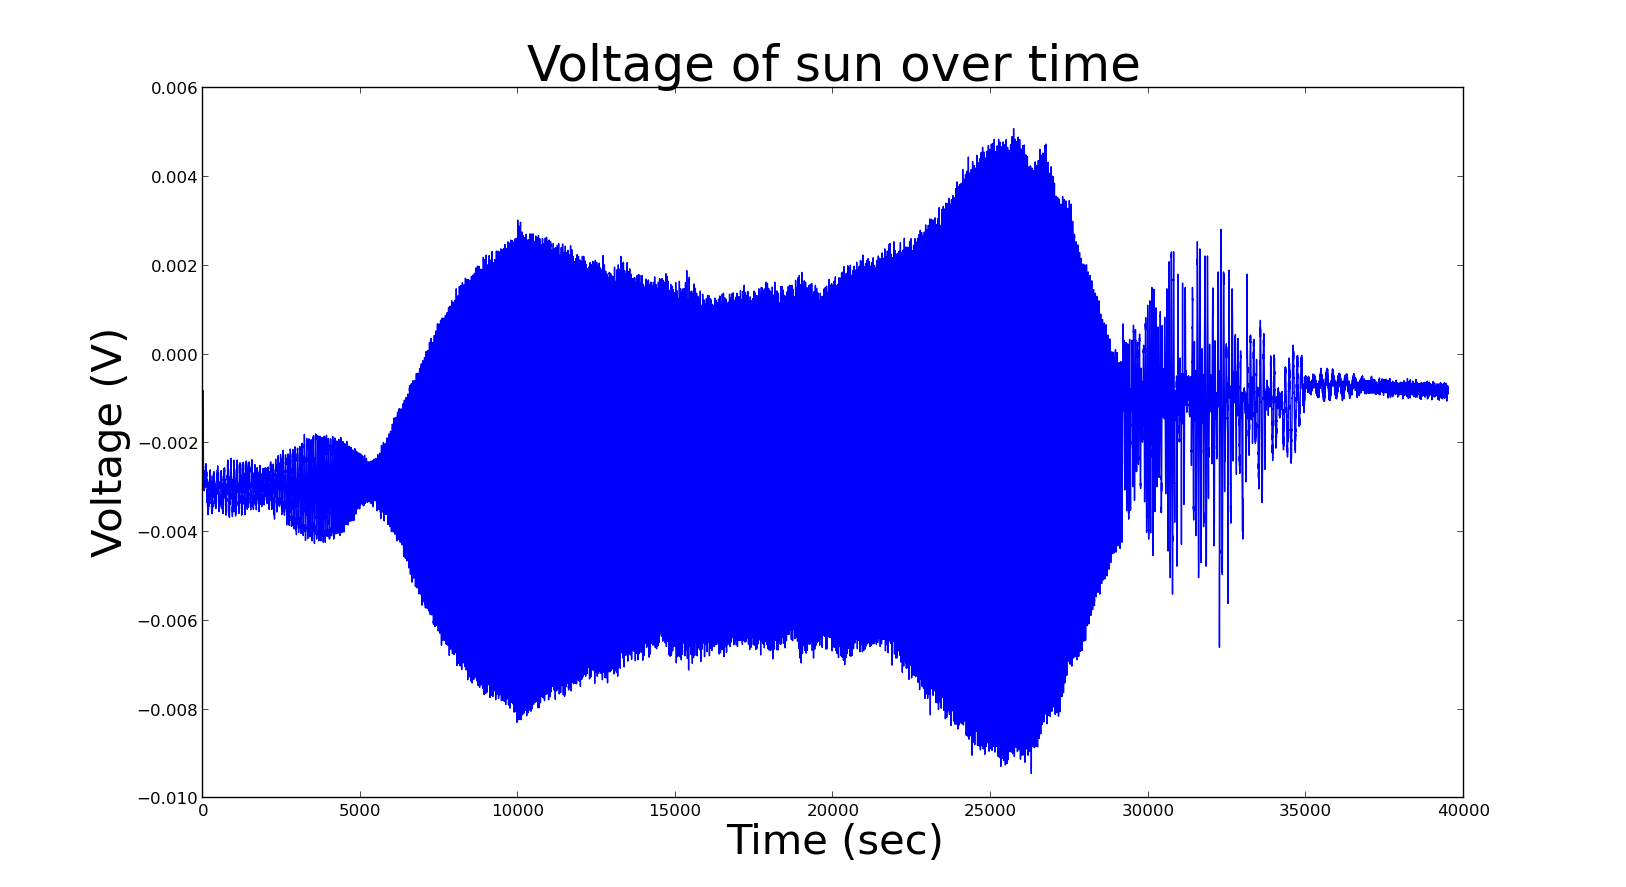
\includegraphics[scale=0.35]{garphs/sundayvolt}
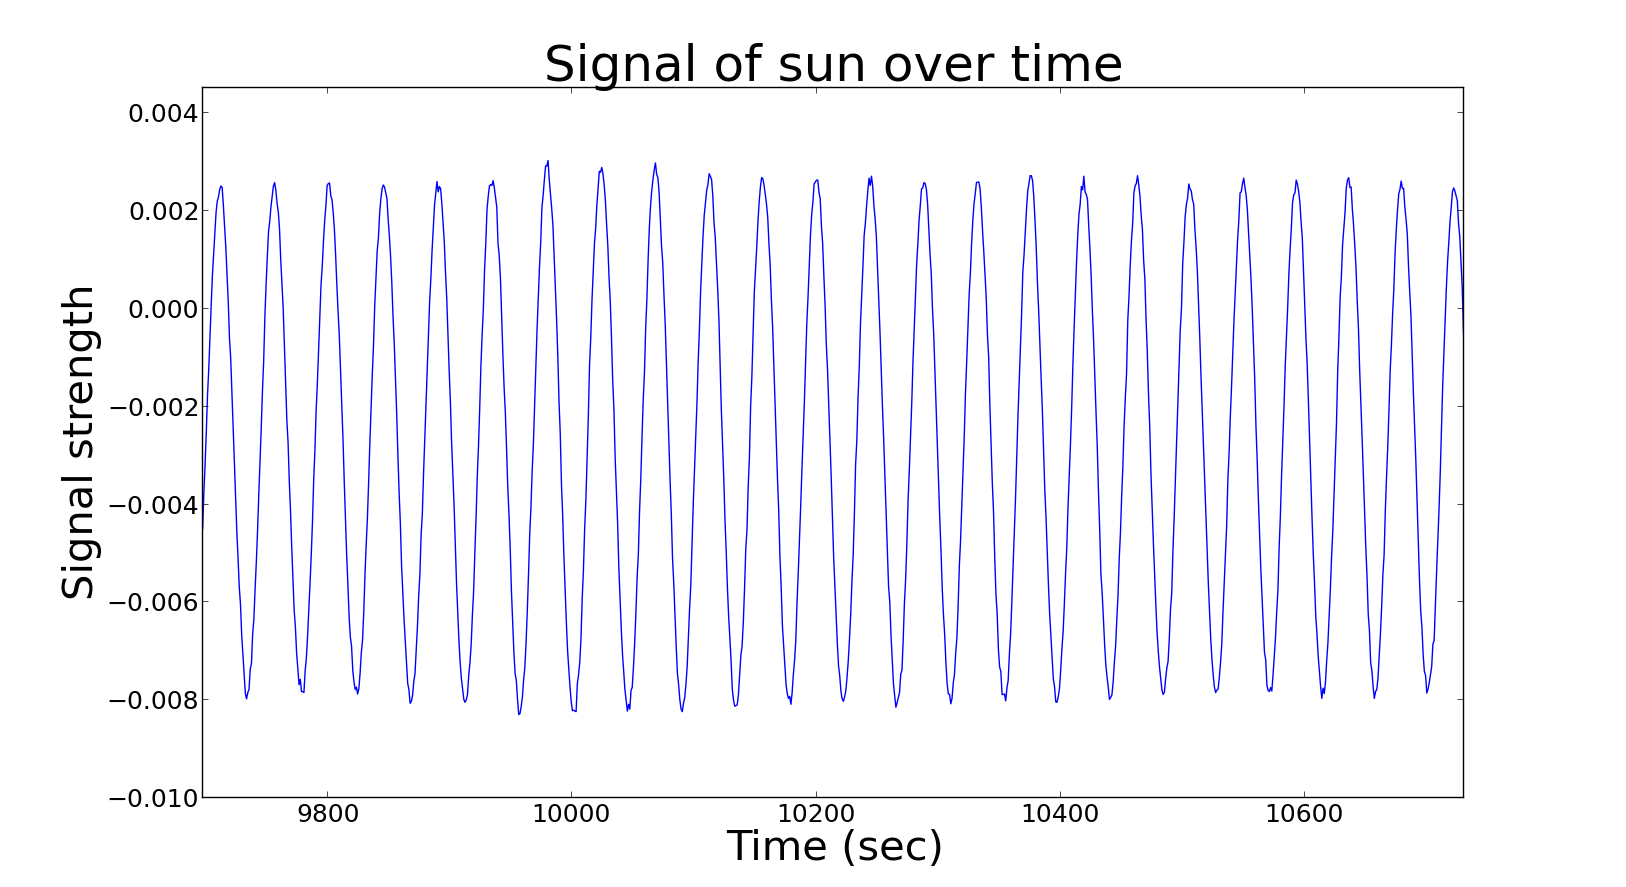
\includegraphics[scale=0.35]{garphs/sundayzoom}
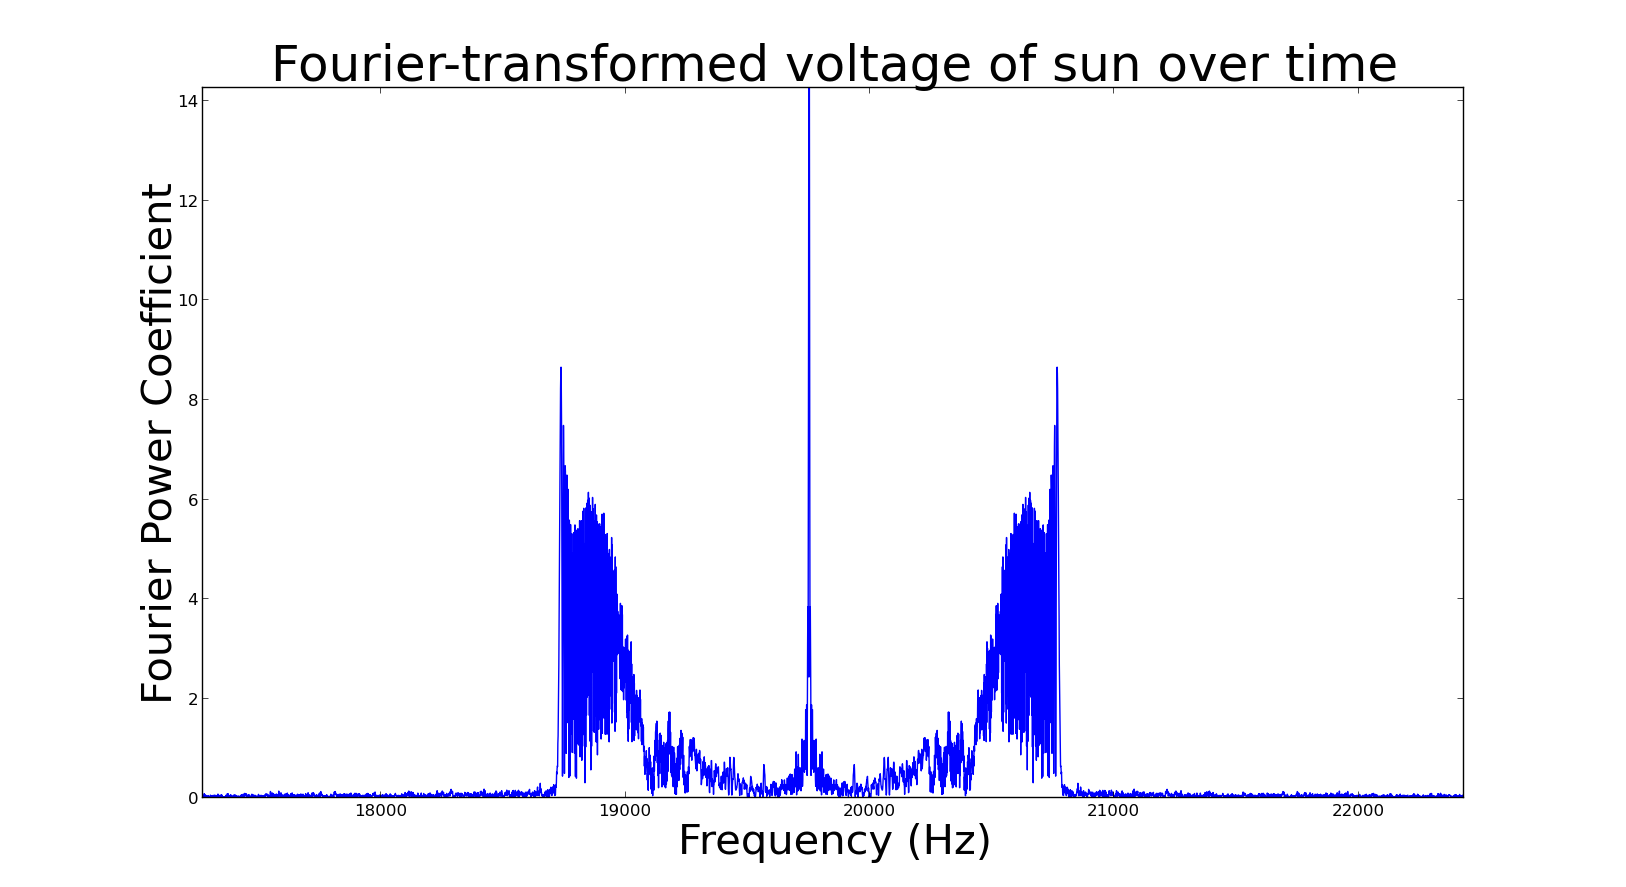
\includegraphics[scale=0.35]{garphs/sundayfourier}
\caption{The top graph shows the signals we measured from the sun over the course of a day. The middle shows a zoomed-in version of this data. The bottom shows the Fourier transform of the top. \label{daysun}}
\end{figure}

The sun's signal comes through as a sinusoid, as we expect from the properties of the interferometer. Looking at the Fourier transform, one can see strong peaks a few thousand Hz past the DC offset in the center. As in the last lab, our Fourier distributions are symmetric about zero due to the complex exponential multiplication that the interferometer does. Using formula 11, we can calculate the expected range of fringe frequencies and compare it with our observed frequencies. Assuming $B_y = 10$m and $\lambda = 2.5$cm, we get $f_f = B_y / \lambda * 2\pi / (86400) = .03\cos{h_s}$ Hz, where $h_s$, the hour angle, varies between $-\pi/2$ and $\pi/2$ throughout the day, being 0 at the meridian. Thus, we can expect that we will see frequencies in the Fourier spectrum between 0 and $.03$ Hz, with the power increasing as we move towards .03, since the sun is strongest at the meridian. This is exactly what we see in the full-day data, and the hour-long data, which was taken around midday, just shows a strong peak around .03 Hz. 

%COMMENT: Using \label{value} and \ref{value} will allow you to refer to
%a specific figure without worrying about the order in which you have
%them in your document. While this obviously matters somewhat in terms
%of the logical flow of you paper, it's really helpful if you're moving
%things around as you write your paper. I did this for the first figure,
%but you can change the rest fairly easily. Additionally, \centering
%will put the figure in the middle of the page when you scale it down to
%a more reasonable size.

%TODO desired ideal filter response, actual calculated filter response

%COMMENT:By placing your figures in the flow of your text, you can
%increase the likelihood that they appear in reasonable places based on
%where you reference them. Combining figures (2 & 3 were combined) that
%are related or demonstrate two aspects of one thing can also allow you
%to use space in your paper more effectively.


%COMMENT: Captions should go below figures always.
\section{Conclusion}

%COMMENT: In a report you don't need to write out unit names, and it
%would actually be preferred you use things like $\mu$H versus mircoHenry

\end{document}
